\section{Broken Symmetry in Quasi-2D Coulomb Systems}

\subsection{Oscillatory single particle field}

The dielectric confinement effect turns out to be physically fascinating even in the presence of a single charged particle. 
In Fig.~\ref{fig:force_x} (a), we present the electric field in the $x$ direction generated by a cation with valence~$\nu=1$ located at~$(x_0, y_0, \tau_0)$ in a quasi-2D system with a thickness of~$10\tau_0$, as a function of the distance from the cation~$\Delta x=x-x_0$, for different reflection rates~$\gamma$ characterizing the confinement. 
The field is defined as~$-\nu\ell_B\partial_x G(\mathbf{r}, \mathbf{r_0})$, where~$G(\mathbf{r}, \mathbf{r_0})$ is given by Eq.~\eqref{eq:G_pv}, and~$\ell_B=e_0^2/(4\pi\epsilon_0\epsilon k_B T)$ is the Bjerrum length of the solvent, with~$e_0$ the elementary charge,~$\epsilon_0$ the vacuum permittivity,~$k_B$ the Boltzmann constant, and~$T$ the temperature. 
For~$\vert\gamma\vert<1$ cases, as illustrated by the blue ($\gamma=-0.95$) and orange ($\gamma=0.95$) lines in Fig.~\ref{fig:force_x} (a), the polarization weakens or enhances the bare Coulomb field ($\gamma=0$), but with no qualitative difference. 
The results obtained by our method are in good agreement with those obtained by ICM, shown in dots in Fig.~\ref{fig:force_x} (a). 
However, for~$\vert\gamma\vert>1$, the results become non-trivial and qualitatively different. 
At short distance ($\tau_0<\Delta x < 10\tau_0$), we observe from Fig.~\ref{fig:force_x}(a) a continuous transition in the the near field interaction from like-charge attraction (LCA) into repulsion as~$\gamma$ increases from $-10$ to $+10$,
which can be understood as a significant enhancement of the polarization effect for~$\abs{\gamma}<1$ cases.
Even more interesting is the far field, it no longer decays monotonically but exhibits oscillatory behavior, which is rarely reported in previous studies.

\begin{figure}[htbp]
	\centering
	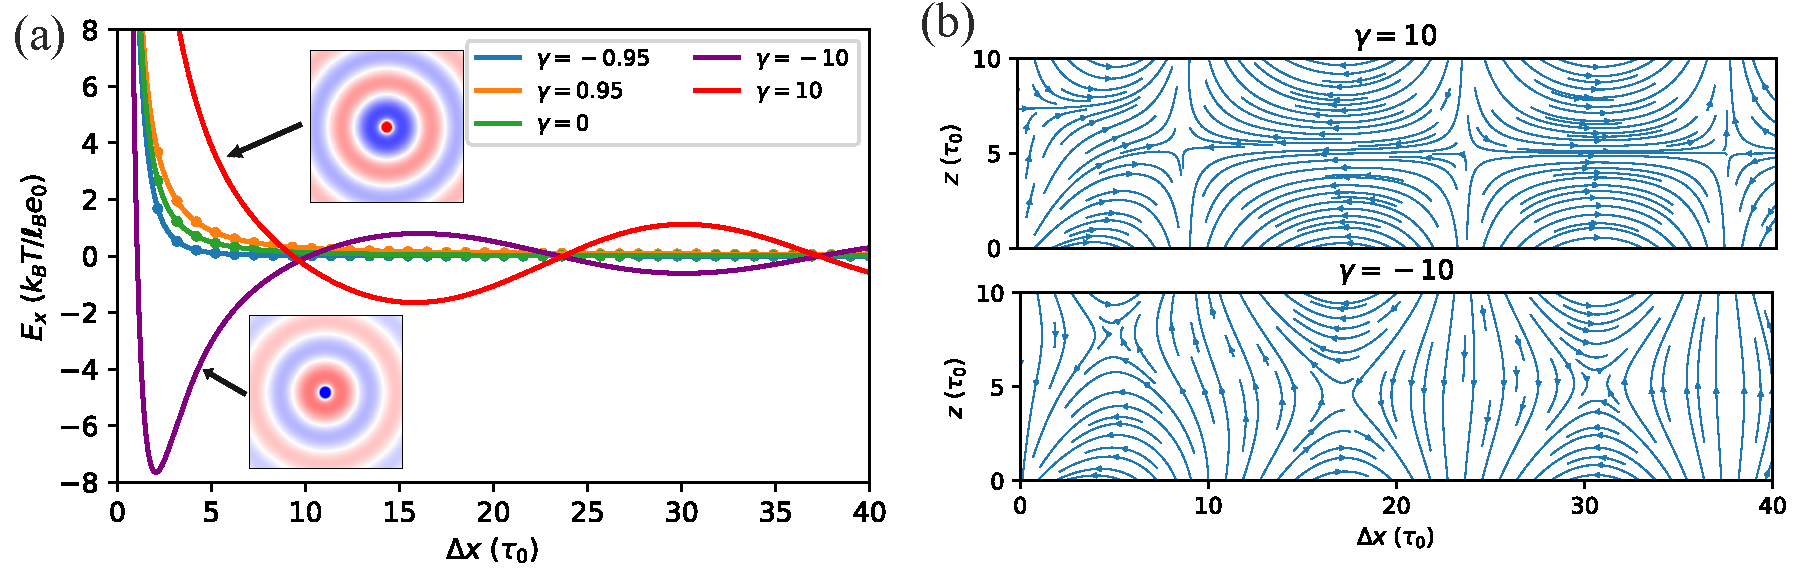
\includegraphics[width=0.45\textwidth]{figs/fig2.pdf}
	\caption{(a): the electric fields along~$x$ direction, generated by a cation with valence~$\nu=1$, fixed at~$z=\tau_0$, and confined by a pair of dielectric substrates located at~$z=0$ and~$10\tau_0$. Subplots depict the polarization charge density on the lower substrates. 
    (b): the corresponding field lines for the~$\gamma=\pm10$ scenarios.
		\label{fig:force_x}
            }
\end{figure}

To understand the origin of field oscillations, the polarization charge density profile on the substrate at~$z=0$ is shown in the subplots of Fig.~\ref{fig:force_x} (a). 
The charge density is defined by 
\begin{equation}
    \sigma(\V{r}) = \lim_{z \to 0^+} \nu \ell_B \eps_0  \left( 1 - \frac{\eps}{\eps'} \right) \partial_z G(\V{r}, \V{r_0})\;,
\end{equation}
and the field lines generated by $\sigma(\V r)$ are sketched in Fig.~\ref{fig:force_x} (b). 
The field oscillation is found to be generated by the strong transverse polarization charge density waves, influencing both the near and far fields. 
The oscillatory field lines has a very similar structure to that of a surface plasmonic resonance wave~\cite{willets2007localized}, but the physical origin is different. 
The oscillation is due to the reflected polarization enhanced by the dielectric confinement, characterized by parameters~$\gamma_1$,~$\gamma_2$, and~$L_z$. Particularly,
The confinement induced oscillation wave number is given by
\begin{equation}\label{eq:k0}
    k_0 = \frac{\ln{\gamma_1 \gamma_2}}{2 L_z}\;,
\end{equation}
which we will show analytically that this corresponds to a first-order pole in the Sommerfeld integral representation of the Green's function.
And the wavelength of the oscillation, defined as two times the distance between nearby zeros, satisfies 
\begin{equation}\label{eq:wavelength}
    \lambda \cdot k_0 = 2 \pi \;.
\end{equation}
Numerical validation shows that Eq.~\eqref{eq:wavelength} is highly robust under different choices of~$\V{r}$,~$\V{r}_0$,~$\gamma$, or~$L_z$, as shown in Fig.~\ref{fig:k_wavelegth}.
Importantly, the oscillation fields can be accurately predicted and controlled by adjusting~$k_0$. 
Eq.~\eqref{eq:k0} also indicates that the oscillation shall be weakened as $L_z$ is increased, and becomes non-oscillatory when $\gamma_1\gamma_2<1$.

\begin{figure}[htbp]
    \centering
    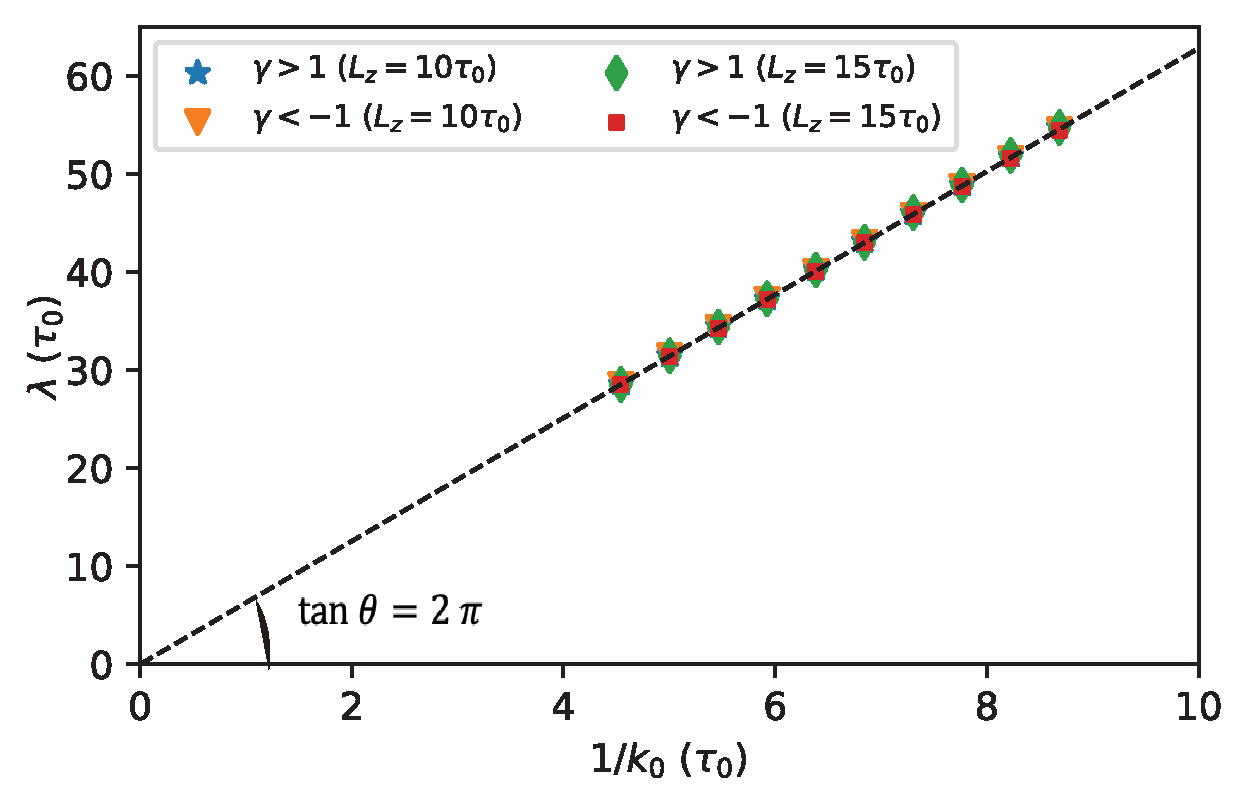
\includegraphics[width=0.6\textwidth]{figs/fig3.pdf}
    \caption{
        Numerical validations for the relationship between~$k_0$ and~$\lambda$ under various system parameter settings of~$\gamma$ and~$L_z$. For each case, $\lambda$ is approximated by averaging distances between nearby zeros of~$E_x$, and with different (randomly generated) locations in~$z$. 
    }
    \label{fig:k_wavelegth}
\end{figure}


\subsection{Theoretical origin for oscillations}

Eq.~\eqref{eq:G_point_charge} shows that the Green's function can be represented as a Sommerfeld integral, and the analytical form of $g(k, z, z_s)$ indicates that it has non-trival behaviors.
Clearly, $g(k, z, z_s)$ is divergent at $k=k_0$ (given in Eq.~\eqref{eq:k0}), and as $\gamma_1\gamma_2$ increases to be larger than 1, $k_0$ will shift onto the positive real axis, then the Sommerfeld integral needs to be renormalized.
Notice that when~$k \to k_0$, the divergent factor has the property
\begin{equation}
    \frac{1}{\gamma_1 \gamma_2 \exp{(-2 k L_z)} - 1} \to \frac{1}{2 L_z (k_0 - k)}\;,
\end{equation}
so that~$k_0$ is a first-order pole and the Cauchy principal value exists.
Then Eq.~\eqref{eq:G_point_charge} for~$\gamma_1 \gamma_2 > 1$ cases is given by
\begin{equation}\label{eq:G_pv}
    G(\V{r}, \V{s}) = - \text{p.v.} \left[ \int_{0}^{+\infty} 2 g(k, z, z_s) J_0(k \Delta \rho) k \text{d}k \right]  \;,
\end{equation}
which can be calculated numerically. In what follows, we analyze the oscillatory behavior~(for more details, see Supplementary Information (SI)~\cite{SI}). First, the Green's function consists of integrals of the following general form
\begin{equation}
    I_o = \int_0^{\infty} \frac{J_0(k \D \rho) \text{e}^{-ka}}{\exp{\left( 2 L_z (k_0 - k) \right)} - 1} \text{d}k\;,
\end{equation}
where~$\D \rho$,~$k_0$ and~$a$ are all positive constants.
We find that~$I_o$ can be further expanded as
\begin{equation}
    I_{o} = \frac{e^{-k_0 a}}{2L_z} \int_0^{\infty} \frac{J_0(k^\prime)}{k_0 \D \rho - k^\prime} \text{d}k^\prime + f(k_0, \D \rho, a),
\end{equation}
where~$k^\prime = k \D \rho$, and~$f(k_0, \D \rho, a)$ is a non-oscillatory analytic function which has minor contribution to~$I_o$.
The first integral term can be understood as a function of~$k_0 \D \rho$, or denoted as~$I_{m} (k_0 \D \rho)$. Clearly, $I_{m}$ is solely controlled by~$k_0$, given different parameters of $\gamma$ and $L_z$.
It is found that the first-order pole in $I_{m}$ provides the oscillatory mode, and we also numerical validated that the wavelength of the oscillation in $I_{m}$ indeed satisfies Eq.~\eqref{eq:wavelength}, which explains our findings.

\subsection{Spontaneous symmetry breaking in confined Coulomb systems}

To investigate the influence of dielectric nanoconfinement on the collective behavior of quasi-2D charged systems, we further developed a collection of numerical techniques to efficiently evaluate the Green's function Eq.~\eqref{eq:G_point_charge}. A novel Ewald-splitting type strategy is proposed, together with renormalization techniques and fast convergent quadrature schemes. All fine details and numerical validations are provided in the SI~\cite{SI}.
Our study focuses on a prototypical quasi-2D charged system, consisting of a binary mixture of charged particles described by the primitive model.
The system comprises~$N/2$ cations and~$N/2$ anions, each with the same diameter~$\tau_0$ and valence~$\pm 1$, resulting in an overall charge-neutral system. 
The Hamiltonian of the system is defined as follows, where~$i$ represents the~$i$-th particle with charge~$q_i$ located at position~$\V{r_i}$:
\begin{equation}
   \mathcal H = \frac{1}{2} \sum_{i,j=1}^{N}{}^\prime q_i q_j \ell_B G(\V r_i, \V r_j) + U_{\mathrm{LJ}}\;,\label{eq:Hamiltonian}
\end{equation}
The sum notation~$\sum_{i,j}{}^\prime$ implies that when~$i=j$, the function~$G(\V r, \V r)$ corresponds to the self-interaction term, and~$U_{\mathrm{LJ}}$ is the shift-truncated Lennard-Jones (LJ) potential energy used to model excluded-volume interactions. 
While this model disregards other important interactions observed in experimental realizations, it enables us to isolate the dielectric confinement effect. 
Similar systems have been studied recently in Refs.~\cite{dos2017simulations,liang2020harmonic,yuan2021particle}.

% two choices, 4 graphs or 3 graphs

\begin{figure}
	\centering
	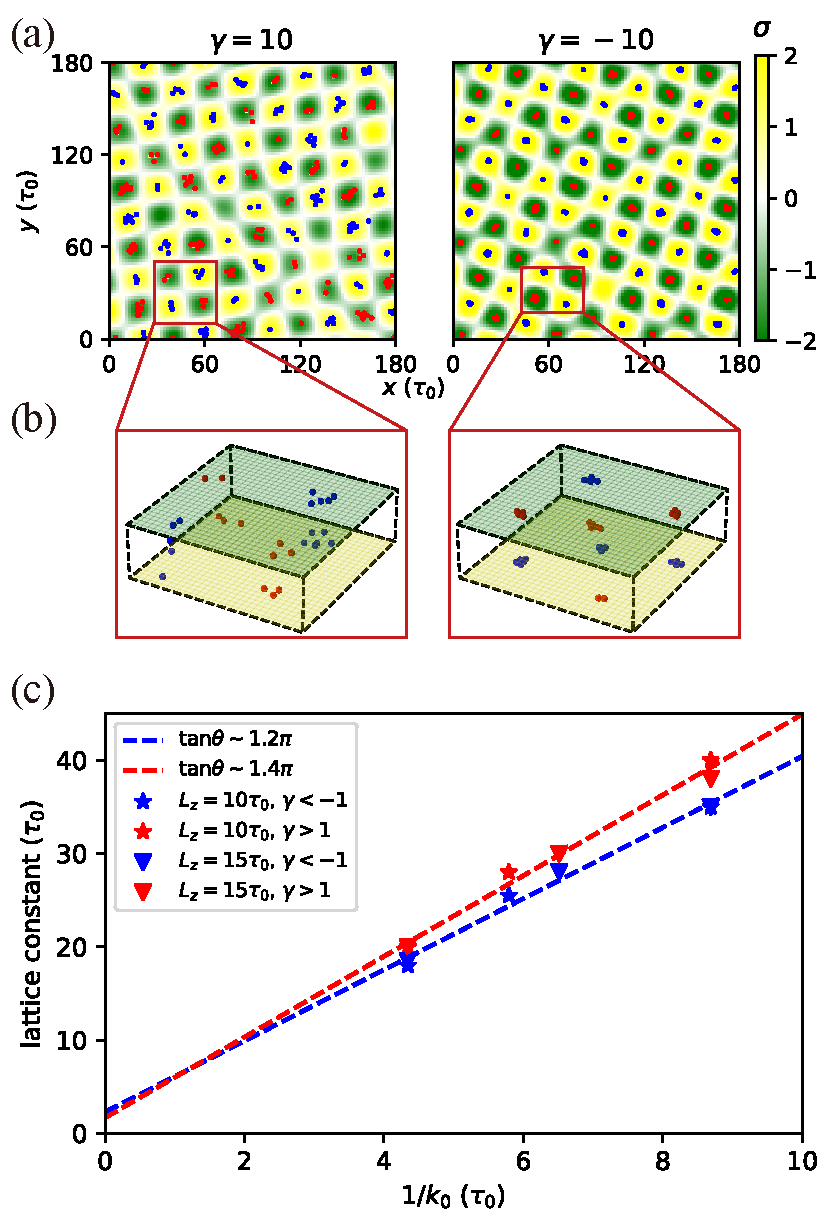
\includegraphics[width=0.43\textwidth]{figs/fig4.pdf}
	\caption{\label{fig:MD} 
        (a): Global particle distributions near the lower substrate and induced surface charge densities for~$\gamma = \pm 10$ and~$L_z = 10$. 
        Positive/negative induced surface charges are in yellow/green, while positive/negative particles are in red/blue, respectively.
        $\sigma$ unit:~$e_0/\tau_0^2$.
        (b): local 3D structures of the charged particles, enlarged from (a), while upper/lower boundaries are in green/yellow, respectively.
        (c): numerical validations for the relationship between the lattice constant and $k_0$. Symbols showing data points from individual simulations, dashed lines depict the linear fitted result.}
\end{figure}

In all the MD simulations, we maintain a constant box size in the~$xy$ plane of~$180\tau_0 \times 180\tau_0$, which is confirmed to eliminate boundary effects.
We vary the values of~$L_z$ and~$\gamma$ to adjust the wave number~$k_0$. 
The system contains~$300$ cations and~$300$ anions.
To isolate electrostatic effect, the reduced temperature $T_r$ is defined as~$T_r =k_{\mathrm B}T/\varepsilon_{\mathrm{Coul}}$, where~$\varepsilon_{\mathrm{Coul}} = e_0^2/(4 \pi \eps (3.5 \tau_0))$ and we set~$\varepsilon_{\mathrm{LJ}} = k_B T$ for both particle-particle and particle-substrate interactions. 
We integrate the temporal evolution using the Velocity-Verlet algorithm and control the temperature using the Anderson thermostat with stochastic collision frequency~$\omega = 0.1$ and reduced temperature~$T_r = 1$.

In the $\abs{\gamma}\leq 1$ regime, extensive simulation works have been done recently~\cite{liang2020harmonic,yuan2021particle} and no SSB phenomenon has been found, i.e., the density distributions of cations $\rho_{+}(\V r)$ and anions $\rho_{-}(\V r)$  always maintain symmetries of the system, given by 1) \emph{cross symmetry} in the confined space: $\rho_{+}(\V r)=\rho_{-}(\V r)$, 2) \emph{longitudinal symmetry}: $\rho_{\pm}(x,y,z)=\rho_{\pm}(x,y,L_z-z)$, and 3) \emph{transverse symmetry}: $\rho_{\pm}(x,y,z)=\rho_{\pm}(x',y',z)$. 
Our simulations give symmetric results for  $\abs{\gamma}\leq 1$, consistent as previous investigations (details are documented in SI~\cite{SI}). 
In the following discussions we will focus on the strongly polarizable cases of $\abs{\gamma}>1$, where SSB phenomena arise.

Fig.~\ref{fig:MD}(a) shows two snapshots for particle distributions near the lower substrate and the corresponding induced surface charge densities, for $\gamma=\pm10$ and $L_z=10$. It clearly shows, for the first time, SSB phenomena in such dielectric confined charged system: both the cross and transverse symmetries are broken when $\gamma=10$; and the remaining longitudinal symmetry is further broken when $\gamma=-10$ (as shown in Fig.~\ref{fig:MD}(b)).

Globally, we observe charged particles spontaneously forming square lattice structures near the substrates for both~$\gamma > 1$ and~$\gamma < -1$ cases, which breaks the transverse symmetry. 
We attribute this to the long-range single particle oscillatory field in the $xy$-plane, which directs particles self-organizing into a \emph{checkerboard} structure, so as to enhance the overall induced charge landscape, which helps confining particles in local potential wells.
Locally within each lattice site, two different particle structures are observed: for~$\gamma >1$, interfacial liquid phase is formed, while for~$\gamma < -1$, likely-charged particles self-assemble into 2D clusters, both can be understood by the near field behaviors due to a single confined particle, as was discussed and illustrated in Fig.~\ref{fig:force_x} (a).

Interestingly, in the longitudinal direction, we find that the interfacial liquids/clusters on opposing substrates are strongly correlated, i.e., there is a one-to-one “pairing” between the opposing particle structures, as show in Fig.~\ref{fig:MD}(b).
For $\gamma=10$, the longitudinal pairing is between symmetrically charged particles; while for $\gamma=-10$, the pairing becomes anti-symmetric, which further breaks the longitudinal symmetry. The symmetric/anti-symmetric longitudinal paring is due to the induced charge landscape on opposing substrates, it is clearly that for $\gamma=10$, the checkerboard structures would be matched symmetrically, while for $\gamma=-10$ a negative sign is added to the reflection rates, forming anti-symmetric pairs.

Finally, it is worth noting that the formed square lattices can be well-controlled via the single parameter~$k_0$, consistent with our theoretical prediction.
As shown in Figure \ref{fig:MD}(c), the lattice constant of the system is found to be proportional to $k_0^{-1}$, with various choice of $L_z$ and $\gamma$. 
Two slightly different linear relationships are observed, with fitted ratio~$1.2 \pi$ and~$1.4 \pi$ for~$\gamma < -1$ and~$\gamma > 1$ cases, respectively. 
The distance between neighboring clusters is found to be consistent with the second zero point of the induced surface charge density profile due to a single point charge (see subplots of Fig.~\ref{fig:force_x} (a)). The mechanism allows one to efficiently modulate the collective phase of dielectric confined systems.